\documentclass[10pt,letterpaper]{article}
\usepackage[T1]{fontenc}
\usepackage[utf8]{inputenc}
\usepackage{lmodern}
\usepackage{microtype}
\usepackage[margin=0.78in,top=0.82in,bottom=0.8in,columnsep=0.27in]{geometry}
\usepackage{amsmath,amssymb,booktabs,array}
\usepackage{graphicx}
\usepackage{tikz}
\usetikzlibrary{arrows.meta,positioning,shapes.geometric}
\usepackage[colorlinks=true,urlcolor=blue!60!black,linkcolor=blue!60!black,citecolor=blue!60!black]{hyperref}
\usepackage{fancyhdr}
\usepackage{enumitem}
\usepackage{xcolor}
\usepackage{multicol}
\usepackage{caption}
\setlist[itemize]{leftmargin=*,nosep,topsep=3pt,parsep=1pt}
\setlength{\parindent}{1em}
\setlength{\parskip}{2.2pt}
\setlength{\columnsep}{0.27in}
\pagestyle{fancy}
\fancyhf{}
\fancyhead[L]{\footnotesize SUPER-GENIUS TECHNICAL MANUSCRIPTS}
\fancyhead[R]{\footnotesize NOVEMBER 2026}
\fancyfoot[C]{\thepage}
\renewcommand{\headrulewidth}{0.35pt}
\newcommand{\figstep}[1]{\tikz[baseline=(X.base)]\node[draw=black!55,rounded corners=2pt,fill=black!3,inner sep=5pt,text width=0.85\columnwidth,align=center,minimum height=0.34in] (X) {\footnotesize #1};}
\newcommand{\sourceline}{\vspace{1pt}\noindent\textit{Scope note:} This manuscript presents an architecture and its analysis. A design description is not an empirical security proof.}

\begin{document}

\begin{center}
{\Large\bfseries Decentralized Verification of Multiparty Computations\\Using Elliptic-Curve Aggregation\par}
\vspace{7pt}
{\normalsize Kenneth Hurley\par}
\vspace{2pt}
{\small \url{https://super-genius.github.io}\par}
\vspace{4pt}
{\footnotesize Independent technical manuscript \quad | \quad Version 1.0 \quad | \quad November 1, 2026}
\end{center}
\begin{abstract}
Decentralized systems must determine whether a collection of participants has produced a valid result without necessarily disclosing each participant's input. This paper describes a proposed verification architecture built around a requestor, elliptic-curve aggregates, and a circuit-oriented transaction validator. It gives the relations checked by a supplied C++ prototype, distinguishes group arithmetic from a complete zero-knowledge proof, and identifies the conditions required for private, independently verifiable execution. The design supports a broader goal of checking distributed transaction or compute results at network boundaries. The accompanying source is a prototype; this paper does not report a production deployment, cryptographic security proof, or performance benchmark.
\end{abstract}
\vspace{3pt}
\noindent\textbf{Keywords:} multiparty computation; elliptic-curve commitments; transaction verification; decentralized systems
\vspace{15pt}
\begin{multicols}{2}

\section{Introduction}
Distributed computation introduces a verification problem: parties can submit intermediate values or results, but peers need a sound way to accept a result despite node failure, disagreement, or malicious input. A direct recomputation may be expensive and can reveal private values. Cryptographic commitments and proofs offer ways to separate the values being checked from the data disclosed to a verifier.

The architecture examined here arose from a proposed decentralized multiparty-computation (MPC) verifier and two C++ modules: \texttt{Requestor} and the MPC verifier circuit. Its narrow implementation concerns transaction aggregates and balance checks. A larger design contemplates distributed proof generation, independent verification, and optional consensus acceptance. We distinguish these layers because arithmetic consistency alone does not establish general MPC correctness or secrecy.

\section{System Model}
Let $P_1,\ldots,P_n$ be participants and let $V$ be a verifier. A requestor initializes parameters, distributes or derives nonce material, and collects an aggregate. A transaction consists of an existing balance $b$, an amount $a$, and a proposed new balance $b'=b-a$. The public verification inputs in the prototype are curve-point commitments and an aggregate point; the circuit marks some scalar values as private inputs.

\begin{center}
\begin{minipage}{\columnwidth}
\centering
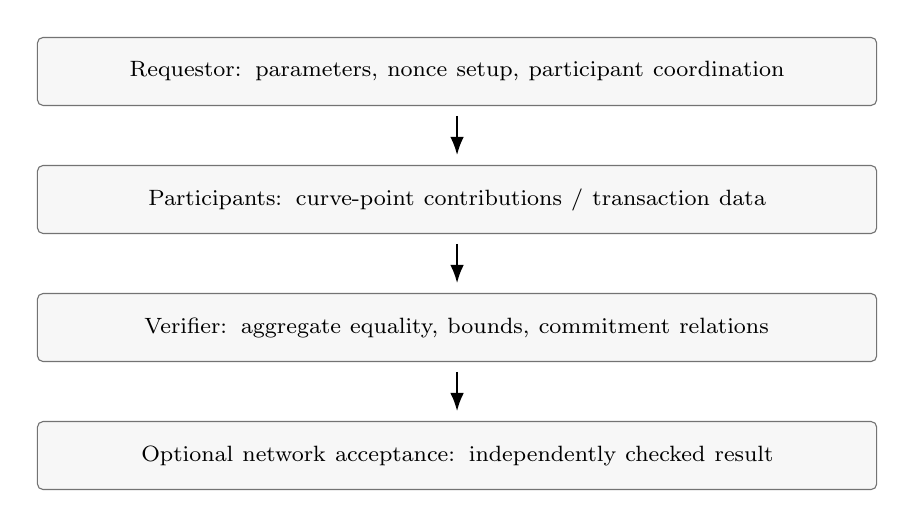
\begin{tikzpicture}[node distance=5mm,>=Latex]
\node (a) {\figstep{Requestor: parameters, nonce setup, participant coordination}};
\node[below=of a] (b) {\figstep{Participants: curve-point contributions / transaction data}};
\node[below=of b] (c) {\figstep{Verifier: aggregate equality, bounds, commitment relations}};
\node[below=of c] (d) {\figstep{Optional network acceptance: independently checked result}};
\draw[->,thick] (a.south)--(b.north); \draw[->,thick] (b.south)--(c.north); \draw[->,thick] (c.south)--(d.north);
\end{tikzpicture}
\captionof{figure}{Logical layers of the proposed verification architecture. The last layer is an integration concept, not demonstrated by the supplied circuit.}
\label{fig:mpcflow}
\end{minipage}
\end{center}

The prototype uses the Pallas elliptic-curve type from the Nil Crypto3 library. Let $G$ denote the chosen curve generator and $\mathbb F_q$ the relevant scalar field. Curve points form an additive group. An expression such as $xG$ denotes scalar multiplication, not a native 256-bit integer accumulator.

\section{Verification Relations}
The supplied \texttt{MPCValidate}\allowbreak\texttt{Transaction} routine returns the conjunction of five checks:
\begin{align}
 A_{\mathrm{out}} &= A_{\mathrm{expected}},\\
 b &\ge a,\\
 C_b &= bG,\\
 C_a &= aG,\\
 C_{b'} &= (b-a)G.
\end{align}
Here $A_{\mathrm{out}}$ is the supplied final aggregate point and $A_{\mathrm{expected}}$ is an expected aggregate point. The inequalities and commitment equalities are explicit in the source. They give a compact transaction consistency test when the caller's inputs and group operations have the intended meaning.

These relations are \emph{not} by themselves a completed zero-knowledge proof. A sound proof implementation must define a proof relation, trusted or transparent setup assumptions, a prover, a verifier, and an exact binding of each public statement to private witnesses. A \texttt{[[circuit]]} annotation indicates design intent but does not prove that those steps are implemented in the files provided.

\subsection{Nonce aggregation}
The requestor constructs two point sequences using a base nonce $\nu$, a node-dependent value $r_i$, a node index $i$, and a block index $j$. In simplified notation, its pair construction has the form
\begin{align}
 N^-_{i,j} &= (\nu-r_i+i+j)G,\\
 N^+_{i,j} &= (\nu+r_i+i+j)G.
\end{align}
Adding one matched pair cancels $r_i$:
\begin{equation}
 N^-_{i,j}+N^+_{i,j}=2(\nu+i+j)G.
\end{equation}
This cancellation is an algebraic property of the construction; it does not hide the inputs against all attacks. It also means the paired total is not simply a sum of the $r_i$ values.

The current requestor stores values across node and block loops, but its \texttt{getFinalAggregate()} iterates over only the first $n$ stored pairs. A separate method computes $2\nu nmG$, where $m$ is the number of blocks per node. These expressions need reconciliation before the aggregate can serve as a reliable public statement.

\section{Privacy and Correctness}
\subsection{Commitment design}
The sample uses $C_v=vG$. For a small amount or balance, a party can enumerate candidate $v$ values and compare points, so this representation alone does not provide strong hiding. A standard blinded alternative is a Pedersen-style commitment,
\begin{equation}
 C_v=vG+rH,
\end{equation}
with independent generators $G,H$ whose discrete-log relation is unknown and a fresh random blinding scalar $r$ \cite{pedersen}. Such a change would require corresponding verification constraints and a correct mechanism for opening or proving relations among commitments.

\subsection{Range and overflow claims}
Embedding a 32-bit or 64-bit value into a 256-bit group does not automatically prevent overflow in an integer calculation. Group arithmetic is modulo the group order. To show that a balance remains nonnegative in ordinary integer arithmetic, a proof must constrain the range of $a$, $b$, and $b-a$, including any carry or wraparound conditions. Efficient range proofs have a substantial prior literature \cite{bulletproofs}.

\subsection{Adversarial nodes}
A verifier should reject stale transcripts, reused nonces, malformed or off-curve points, inconsistent participant identities, unauthorized changes to the accepted statement, and aggregates assembled from incomplete participant sets. Proofs should bind to a request identifier, participant set, network identifier, and fresh challenge. Cryptographic nonce material must come from a cryptographically secure source. The prototype uses \texttt{std::mt19937}, which is appropriate for simulation but not secret cryptographic randomness.

\section{Distributed Protocol}
A complete protocol can be organized into four stages. First, the requestor establishes a signed request context and a precisely defined algebraic statement. Second, participants submit authenticated contributions and, where needed, encrypted or committed private values. Third, a proof system produces evidence that valid contributions imply a result satisfying the stated arithmetic and policy constraints. Fourth, an independent verifier checks the proof and authorizes the network to accept or reject the result.

The precise proof system remains an engineering choice. Circuit-based proofs could use existing succinct-proof systems, while simpler arithmetic relations may admit specialized sigma protocols or range proofs. Proof construction should reuse audited primitives rather than rely on new cryptographic assumptions.

\section{Evaluation Plan and Implementation Status}
The available test file proposes five cases: a valid transfer, insufficient balance, invalid commitments, a zero-valued transfer, and a transfer equal to the full balance. Tests are useful for exercising the Boolean predicate, but no results, timings, proof sizes, or network measurements were supplied. The following evaluation should precede any empirical claims.

\begin{center}
\begin{minipage}{\columnwidth}
\centering\small
\begin{tabular}{p{0.27\columnwidth}p{0.60\columnwidth}}
\toprule
Measure & Required observation\\
\midrule
Correctness & Pass/fail across ordinary and adversarial inputs\\
Scalability & Cost as participants and blocks grow\\
Proof cost & Prover time, verifier time, proof bytes\\
Fault behavior & Dropped nodes, reordered messages, replay\\
Privacy & Witness leakage and linkability analysis\\
\bottomrule
\end{tabular}
\captionof{table}{Measurements needed to turn the design into a quantified evaluation.}
\end{minipage}
\end{center}

Before those measurements, the prototype needs a valid library-provided curve generator, consistent aggregation indices and formulas, secure randomness, and a concrete proof-generation and proof-verification path. All conclusions in this manuscript are therefore architectural and algebraic rather than empirical.

\section{Distributed Compute Uses}
In a decentralized compute system, verifiable arithmetic could support job settlement, quota tracking, resource accounting, or signed acceptance records. It does not establish that an arbitrary AI answer is factually correct or that arbitrary unproved computation was executed faithfully. Each application must define the property being proved and how the public result binds to the original job.

\section{Conclusion}
The requestor and circuit modules illustrate an approach for checking aggregate and transaction consistency with elliptic-curve operations. The next step is a precise security relation and a working proof system, followed by testing across adversarial network conditions. A limited, accurately stated verifier is more useful than an unverified claim of general MPC correctness.

\end{multicols}
\vspace{6pt}
\begin{thebibliography}{99}

\bibitem{pedersen} T. P. Pedersen, ``Non-interactive and information-theoretic secure verifiable secret sharing,'' in \emph{Advances in Cryptology---CRYPTO '91}, 1992.
\bibitem{bulletproofs} B. B\"unz et al., ``Bulletproofs: Short proofs for confidential transactions and more,'' in \emph{IEEE Symposium on Security and Privacy}, 2018.
\bibitem{shamir} A. Shamir, ``How to share a secret,'' \emph{Communications of the ACM}, vol. 22, no. 11, 1979.
\bibitem{pallas} Electric Coin Company, ``The Pasta curves for Halo 2 and beyond,'' technical documentation, 2020.
\bibitem{source} K. Hurley, \emph{MPCVerifierCircuit.cpp}, \emph{Requestor.cpp}, and accompanying test and header files, author-provided prototype, 2024--2025.

\end{thebibliography}
\vspace{8pt}
\noindent\rule{\textwidth}{0.3pt}
\noindent\footnotesize Prepared for publication at \url{https://super-genius.github.io}. This work is a technical exposition, not a claim of independent certification or completed performance evaluation.
\end{document}
